\documentclass[a4paper,11pt]{article}
\usepackage{amsmath,amsthm,amsfonts,amssymb,amscd,amstext,vmargin,graphics,graphicx,tabularx,multicol} 
\usepackage[francais]{babel}
\usepackage[utf8]{inputenc}  
\usepackage[T1]{fontenc} 
\usepackage{pstricks-add,tikz,tkz-tab,variations}
\usepackage[autolanguage,np]{numprint} 

\setmarginsrb{1.5cm}{0.5cm}{1cm}{0.5cm}{0cm}{0cm}{0cm}{0cm} %Gauche, haut, droite, haut
\newcounter{numexo}
\newcommand{\exo}[1]{\stepcounter{numexo}\noindent{\bf Exercice~\thenumexo} : \marginpar{\hfill /#1}}
\reversemarginpar


\newcounter{enumtabi}
\newcounter{enumtaba}
\newcommand{\q}{\stepcounter{enumtabi} \theenumtabi.  }
\newcommand{\qa}{\stepcounter{enumtaba} (\alph{enumtaba}) }
\newcommand{\initq}{\setcounter{enumtabi}{0}}
\newcommand{\initqa}{\setcounter{enumtaba}{0}}

\newcommand{\be}{\begin{enumerate}}
\newcommand{\ee}{\end{enumerate}}
\newcommand{\bi}{\begin{itemize}}
\newcommand{\ei}{\end{itemize}}
\newcommand{\bp}{\begin{pspicture*}}
\newcommand{\ep}{\end{pspicture*}}
\newcommand{\bt}{\begin{tabular}}
\newcommand{\et}{\end{tabular}}
\renewcommand{\tabularxcolumn}[1]{>{\centering}m{#1}} %(colonne m{} centrée, au lieu de p par défault) 
\newcommand{\tnl}{\tabularnewline}

\newcommand{\trait}{\noindent \rule{\linewidth}{0.2mm}}
\newcommand{\hs}[1]{\hspace{#1}}
\newcommand{\vs}[1]{\vspace{#1}}

\newcommand{\N}{\mathbb{N}}
\newcommand{\Z}{\mathbb{Z}}
\newcommand{\R}{\mathbb{R}}
\newcommand{\C}{\mathbb{C}}
\newcommand{\Dcal}{\mathcal{D}}
\newcommand{\Ccal}{\mathcal{C}}
\newcommand{\mc}{\mathcal}

\newcommand{\vect}[1]{\overrightarrow{#1}}
\newcommand{\ds}{\displaystyle}
\newcommand{\eq}{\quad \Leftrightarrow \quad}
\newcommand{\vecti}{\vec{\imath}}
\newcommand{\vectj}{\vec{\jmath}}
\newcommand{\Oij}{(O;\vec{\imath}, \vec{\jmath})}
\newcommand{\OIJ}{(O;I,J)}

\newcommand{\bmul}[1]{\begin{multicols}{#1}}
\newcommand{\emul}{\end{multicols}}

\newcommand{\reponse}[1][1]{%
\multido{}{#1}{\makebox[\linewidth]{\rule[0pt]{0pt}{20pt}\dotfill}
}}

\newcommand{\titre}[5] 
% #1: titre #2: haut gauche #3: bas gauche #4: haut droite #5: bas droite
{
\noindent #2 \hfill #4 \\
#3 \hfill #5

\vspace{-1.6cm}

\begin{center}\rule{6cm}{0.5mm}\end{center}
\vspace{0.2cm}
\begin{center}{\large{\textbf{#1}}}\end{center}
\begin{center}\rule{6cm}{0.5mm}\end{center}
}



\begin{document}




\exo

\bmul{2}
Convertir les nombres suivants dans l'unité demandée :\\

13,80 m  = ...............................  cm \\

45 mm  = ...............................  m \\

24,5 km  = ...............................  dm \\

6 372 dam  = ...............................  km \\

\columnbreak

 Compléter avec l'unité qui convient :\\
 
500 dm  =   50 ............................... \\

0,7 dm  =    7 ............................... \\

0,09 dam  =   90 ............................... \\

500 000 m  =   500 ...............................\\ 


\emul


\vspace*{1cm}



\exo

\bmul{2}

\includegraphics[scale=0.8]{figperimetrecompte.eps} 

\columnbreak

Observer   attentivement   l'unité   de   longueur (1 u.l.) puis déterminer le périmètre, en unités de longueur, de chaque figure.\\

\noindent \reponse[4]
\emul


\exo \\

\q Calculer le périmètre d'un rectangle MLKJ tel que ML = 9 m et LK = 5,3 m. \\


\q Calculer le périmètre d'un carré OLKI tel que OL = 7,5 cm.  \\



\exo 

Calculer le périmètre des figures suivantes : \\

\bmul{2}

\includegraphics[scale=0.7]{fig1perimetre.eps} 
\columnbreak

\includegraphics[scale=0.7]{fig2perimetre.eps} 

\emul

\color{red}
\textbf{CORRECTION Figure 1:}\\
La figure est un polygone. Son périmètre est donc la somme de ses côtés.\\
2,8 cm = 28 mm\\

$P_{1}= 17,4 \times 2 + 11,7 \times 2 + 28$ 
\fbox{$P_{1}= 86,2 mm$ }


\textbf{CORRECTION Figure 2:}\\
La figure est un polygone. Son périmètre est donc la somme de ses côtés.\\
20 mm = 2 cm  et   0,19 dm = 1,9 cm\\	

$P_{2}= 1,7 + 1,8 + 2 + 1,9$ 
\fbox{$P_{2}= 7,4 cm$ }

\color{black}
\newpage



\exo

Calculer le périmètre des figures suivantes : 


\includegraphics[scale=0.8]{fig4.eps} 





\vspace*{0.5cm}

\color{red}
\textbf{CORRECTION Figure 1:}\\

La figure est composée de 2 segments de même longueur et d'un demi cercle de rayon 2,5 cm.\\

- Les segments :\\

$P_{segments} = 2 \times 2,5$\\

$P_{segments} = 5 $ cm\\



- Le demi-cercle : 

Pour calculer le périmètre d'un demi-cercle, on va calculer le périmètre d'un cercle et le diviser par 2. On peut aussi multiplier $\pi$ par le rayon.
\bmul{2}

$P_{cercle} = 2 \times \pi \times r $\\

$P_{cercle} = 2 \times \pi \times 2,5 $\\

$P_{cercle} \approx 2 \times 3,14 \times 2,5 $\\

$P_{cercle} \approx 15,7$ cm\\

\columnbreak

$P_{demi-cercle} \approx 15,7 \div 2$\\

$P_{demi-cercle} \approx 7,85$ cm\\

\emul



$P_{TOTAL} = P_{segments} + P_{demi-cercle} $\\

$P_{TOTAL} \approx 5 + 7,85 $\\

\fbox{$P_{TOTAL} \approx 12,85 $ cm} \\

Le périmètre de la figure est donc d'environ 12,85 cm.

\color{black}

\includegraphics[scale=0.7]{fig4perimetre.eps} 

\color{red}
\textbf{CORRECTION Figure 2:}\\

La figure est composée de 4 quarts de cercle de rayon 3 cm chacun, ces 4 quarts de cercle forment donc un cercle de rayon 3cm.\\



$P_{cercle} = 2 \times \pi \times r $\\

$P_{cercle} = 2 \times \pi \times 1,5 $\\

$P_{cercle} \approx 2 \times 3,14 \times 1,5 $\\

$P_{cercle} \approx 9,42$ cm\\

Le périmètre de la figure est donc d'environ 9,42 cm.

\color{black}

\newpage

\exo

Calculer le périmètre de la figure suivante :

\begin{center}
\includegraphics[scale=0.6]{fig6.eps} 
\end{center}





\end{document}
